\chapter{Assessment of Transcriptional Induction of Bovine IFITs in the Context of RSV} \label{ch:Assessment of Transcriptional Induction of Bovine IFITs in the Context of RSV}
\section{Introduction and Aims} \label{sec:Introduction and Aims Chapter2}
\textbf{Half page intro:}
Ifit gene regulation (promoters and such) \newline
Ifit paths of induction \newline
interferons \newline
Lps tlr4 \newline
about cross species interaction + question about lab attenuated or not the brsv stuff

\lipsum[1-2]

\textbf{Half page aims:}
We hypothesised  bovine IFITs to be induced by human and bovine RSV infection. We aimed to systematically test this by initially confirming that our model cell lines are capable of IFIT induction following the treatment of known innate immune system activators such as interferon alpha, and LPS. We would then assess the IFIT induction during human and bovine RSV infection using a range of viral concentration and end assay time points. Lastly, we would validate this data in more physiologically relevant cell lines as well as using omics approaches.

\lipsum[1]

\section{Results} \label{sec:Results Chapter2}
\subsection{Technology Establishment} \label{subsec:Technology Establishment}
\subsubsection{Primer Design and Validation for Bovine \textit{IFIT} Quantification} \label{Primer Design and Validation for Bovine IFIT Quantification}
Due to the initial lack of commercially available primers for the detection of bovine \textit{IFIT} transcripts at the outset of the project, I devised a panel comprising three primer sets (PS) for each bovine \textit{IFIT} gene. Detailed information about this process is outlined in Section \ref{subsec:Primer Design and Assay Setup}. In a nutshell, I inputted the coding sequences into the PrimerQuest software (Integrated DNA Technologies) to identify the most suitable oligonucleotides. To evaluate the amplification efficiencies of each primer set, I employed \textit{IFIT} DNA clones from a bovine ISG library as standards (accessible through a collaboration with CVR Glasgow). The outcomes are depicted in Figure \ref{fig:Validation of custom-made bIFIT qPCR primers}. The graph demonstrates that primer sets 1 exhibited the most favourable amplification efficiencies. All primer sets, except for \textit{bIFIT3}, yielded nearly impeccable amplification efficiencies of around 100\%. Consequently, they were chosen for subsequent experiments. While \textit{bIFIT3} primer sets demonstrated similar outcomes in terms of standard curve slopes and amplification efficiencies, PS1 consistently outperformed the others in repeated testing rounds (data not presented). As a result, it was singled out for further experimentation.

\begin{figure}
    \centering
    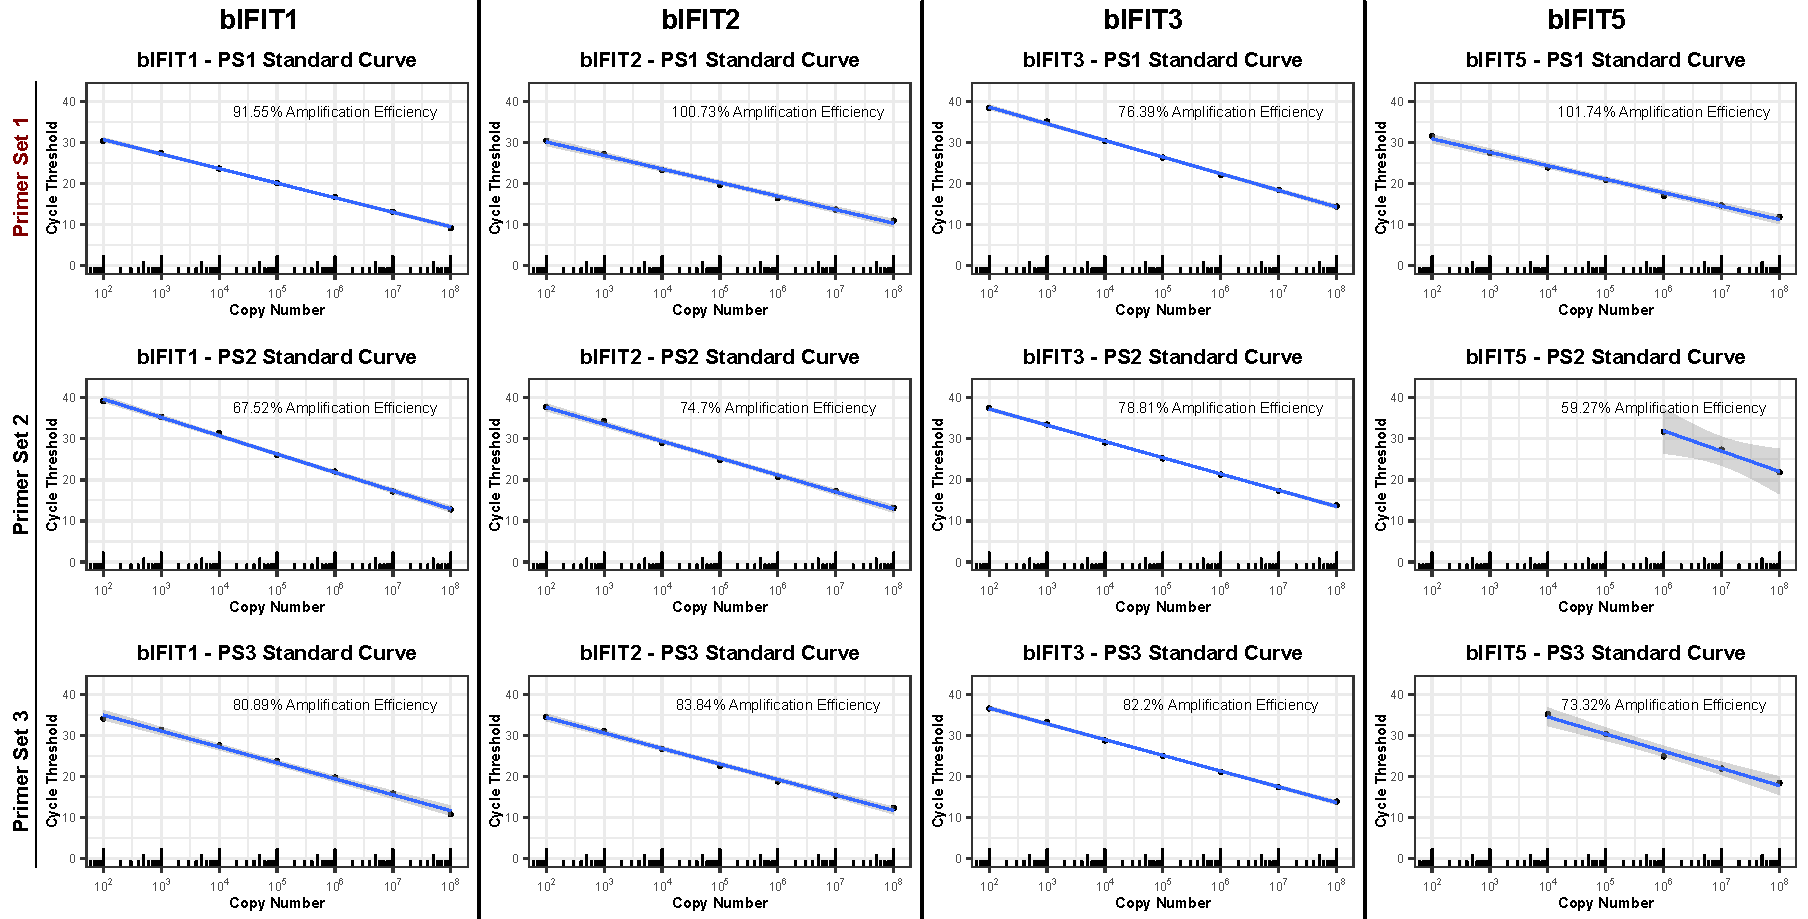
\includegraphics[width=1\linewidth]{07. Chapter 2/Figs/01. Technologies/02. primer validation.pdf}
    \caption[Validation of Custom-Made \textit{bIFIT} qPCR Primers.]{\textbf{Validation of Custom-Made \textit{bIFIT} qPCR Primers.} The custom-designed primers were evaluated by creating a serial dilution of bovine \textit{IFIT}-containing plasmids, provided by the CVR Glasgow. The resulting standard curves are shown here. Primer set (PS) 1 (a), 2 (b), and 3 (c) are depicted for bovine \textit{IFIT1} (1.), \textit{IFIT2} (2.), \textit{IFIT3} (3.), and \textit{IFIT5} (4.), along with their calculated amplification efficiencies.}
    \label{fig:Validation of custom-made bIFIT qPCR primers}
\end{figure}

The PSs behaviour was monitored throughout the project, as fresh standard curves were created per experiment. Figure \ref{fig:The Performance of Custom Made Primer Sets Over Time} shows that the average data is consistent with what was observed in initial testing (Figure \ref{fig:Validation of custom-made bIFIT qPCR primers}), however, there were per experiment deviations in slope angles for each of the selected primer pairs. The underlying amplification efficiencies stayed consistent, as is highlighted by the averaged efficiencies displayed. The initial \textit{bIFIT3} PSs differential amplification slopes compared to the other \textit{bIFIT} PSs, as well as the variable nature of PSs performance throughout the project prohibits the usage of \(\Delta\)\(\Delta\)Ct methodologies for transcript quantification as the increase in cycle threshold would not be proportional to the decrease of transcript abundance between the \textit{bIFITs}, and thus a different methodology had to be adopted. This is described in detail in Section \ref{subsec:Data Processing}. In short, the copy numbers were deducted from standard curves and factorised by the relative abundance of bovine \textit{GAPDH}. This ensured the slope-independent establishment of relative expression values, mirroring and complementing data from \(\Delta\)\(\Delta\)Ct methodologies.

\begin{figure}
    \centering
    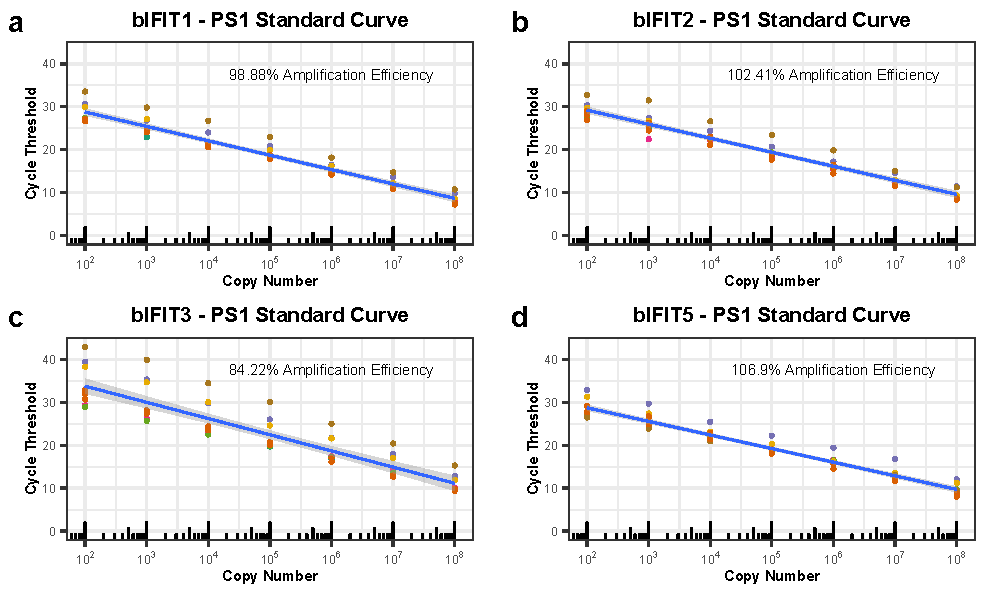
\includegraphics[width=1\linewidth]{07. Chapter 2/Figs/01. Technologies/03. standard curves behaviour.pdf}
    \caption[The Performance of Custom-Made Primer-Sets Over Time.]{\textbf{The Performance of Custom-Made Primer-Sets Over Time.} During the experiments with custom-made \textit{bIFIT} qPCR primers, standard curves had to be always constructed. Here, the underlying average amplification efficiencies and standard curves, along with the individual data, from all the experiments and coloured by the experiment are displayed.}
    \label{fig:The Performance of Custom Made Primer Sets Over Time}
\end{figure}

\subsubsection{Growth Curves of Bovine RSV in Bovine Cell Lines} \label{Growth Curves of Bovine RSV in Bovine Cell Lines}
Although my colleagues in the Viral Glycoproteins Group from the Pirbright Institute routinely perform hRSV infections of the MDBK cell line, the data in the BT cell line is currently lacking. Therefore I set up bRSV growth curves in both cell lines side by side to investigate which time points would be relevant for further infection experiments. Crude-extracted bRSV, isolated as described in Section \ref{subsec:Virus Propagation and Production} and quantified as described in Section \ref{subsec:Virus Quantification by TCID50 Assay} was used for the establishment of growth curves as described in Section \ref{subsec:Viral Growth Curves}. In brief, the MDBK and the BT cell line were seeded in 96-well plates and infected with WT bRSV at MOI 0.1. The supernatant and cellular fractions were collected at time intervals of 24, 48, 72, 96, 120, 144, and 168 hours post-infection, snap frozen in dry ice ethanol mixture, and later tittered as described in Section \ref{subsec:Virus Quantification by TCID50 Assay}. As can be observed in Figure \ref{fig:bRSV growth curves in MDBK and BT cell lines}, there is a differential infection profile between the cell lines. bRSV growth in the MDBK cell line was initially exponential, starting at \(10^{2.5}\) viral titre solely detected in the cytosolic fraction at 24 HPI, it increased to \(10^{4}\) and \(10^{3}\) for the cellular and supernatant fractions respectively at 48 hours. At 72 hours, the cellular viral titre reached \(10^{4.5}\), while the supernatant one further increased to \(10^{3.5}\). Afterwards, the cellular titre remained stable until 120 hours, after which it declined by more than an order of magnitude to \(10^{3}\) at 144 hours and then further increased again to \(10^{3.5}\) at 168 hours. The supernatant titre increased to \(10^{4.5}\) and \(10^{5.5}\) at 120 and 144 hours respectively, and afterwards it decreased to \(10^{4.5}\) again at 168 hours. The peak combined titre occurred at 144 hours but it was robust from 48 hours onwards. bRSV growth in BT cell line displayed virtually no titre from supernatant fraction at 24 and 48 hours. Regardless, the 24-hour time point was the peak value of the combined, as well as cellular titre with cellular titres of \(10^{4}\) at 24 hours and \(10^{3}\) at 48 hours. Cellular titres further declined to \(10^{2}\) at 72 hours, and since then they remained stable other than a small increase to \(10^{2.5}\) at 120 HPI. On the other hand, supernatant titre peaked at 72 hours at \(10^{4}\), slightly decreased to \(10^{3.5}\) at 120 hours and afterwards stayed stable until the end of the experiment. From this experiment, we can conclude that the viral replication kinetics differ substantially between the two cell lines and the data suggests that we can be certain of viral replication at 48 HPI in MDBK cell line and 24 HPI in the BT cell line.

\begin{figure}
    \centering
    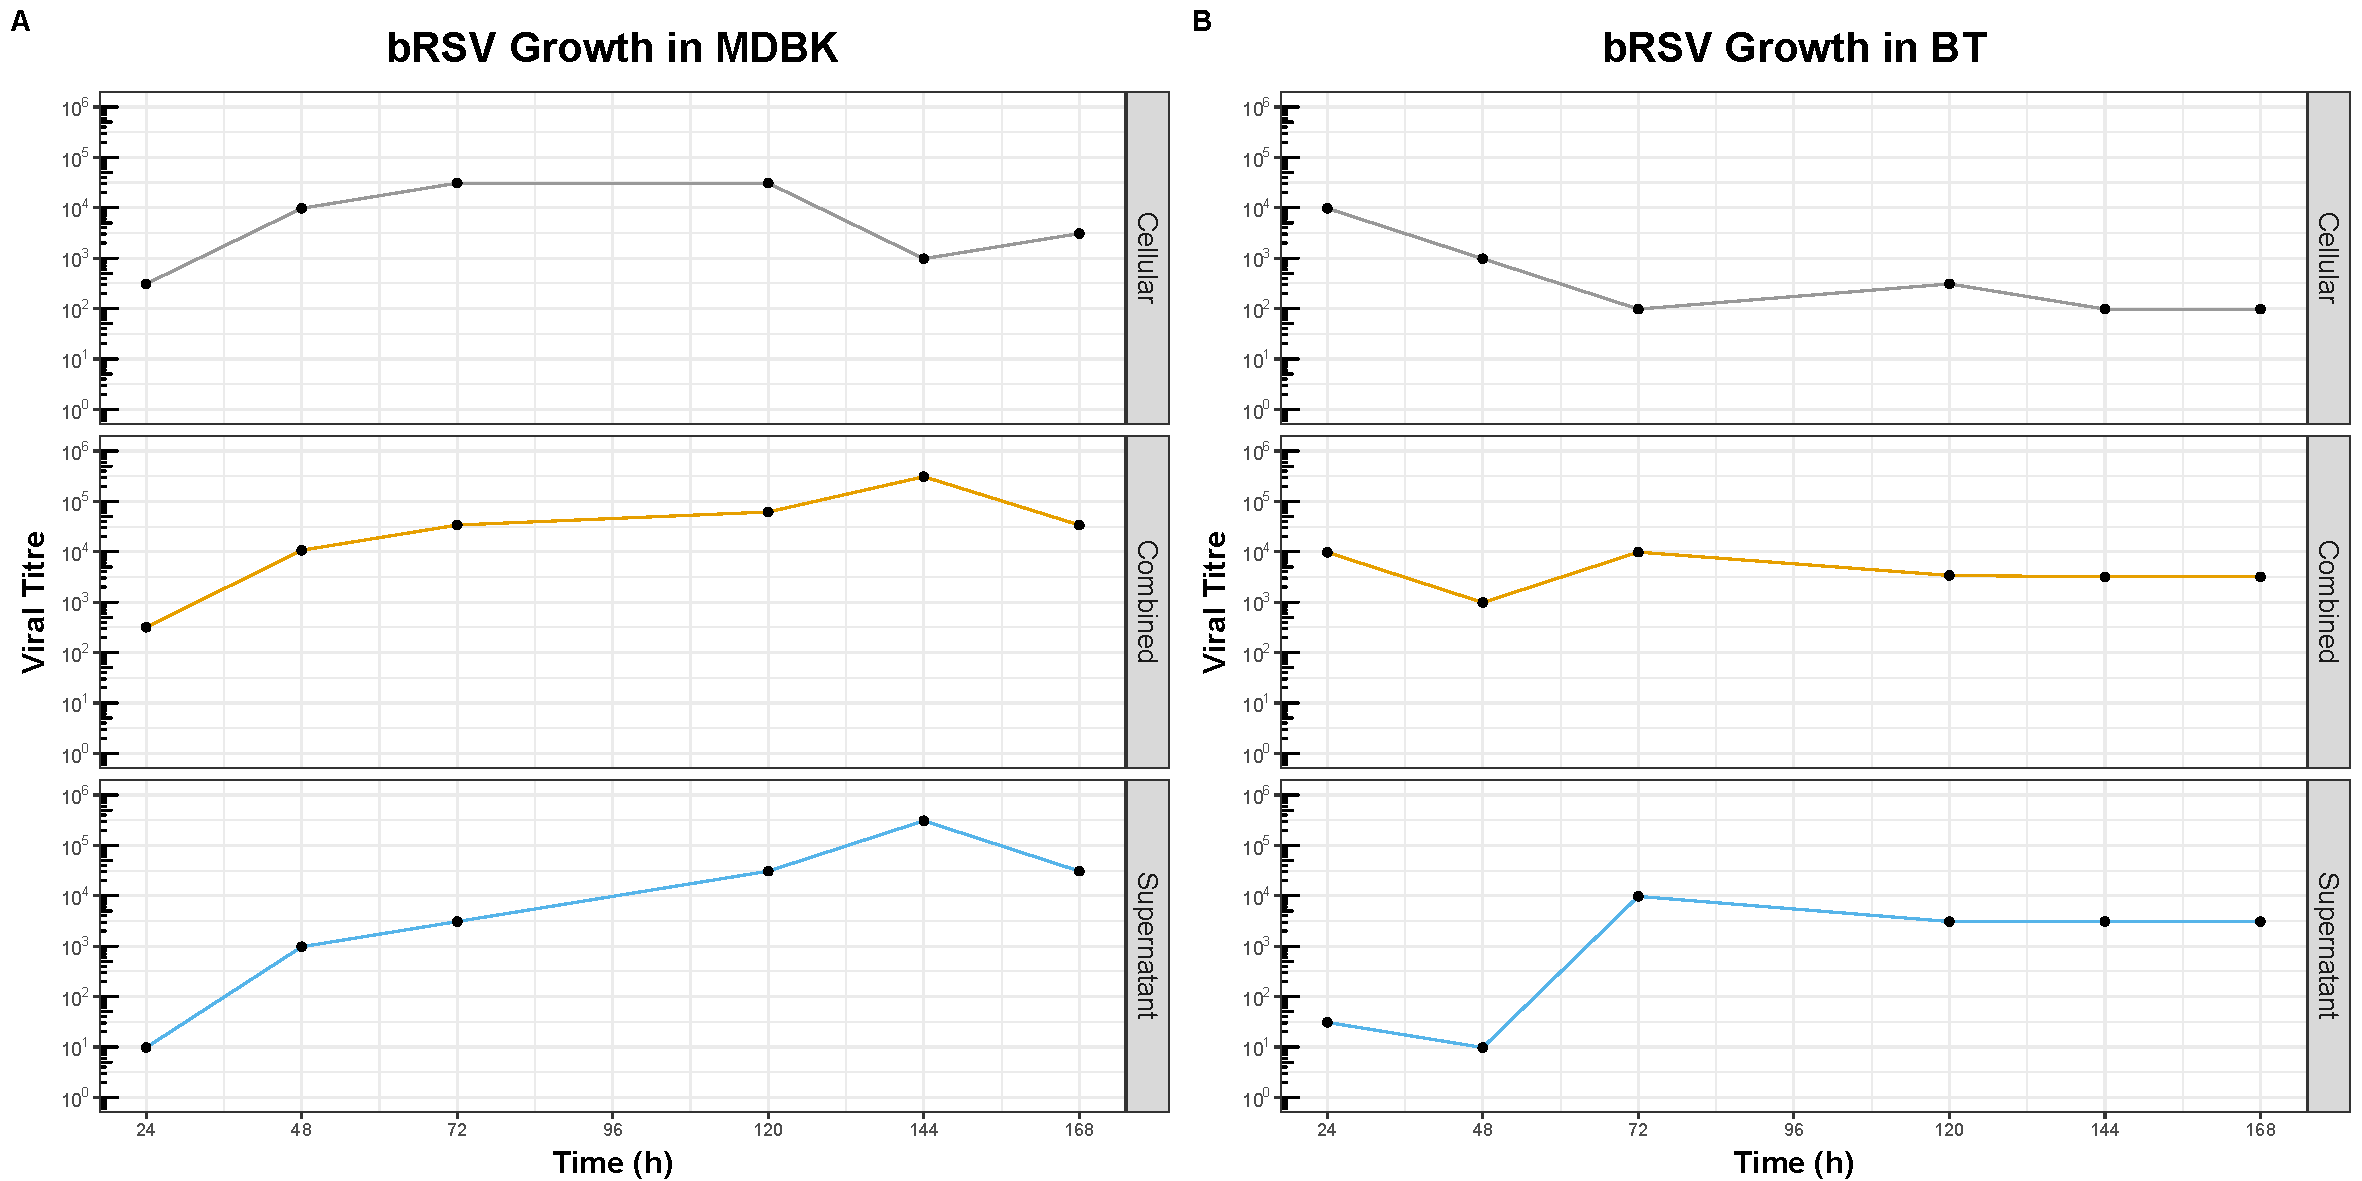
\includegraphics[width=1\linewidth]{07. Chapter 2/Figs/01. Technologies/01. growth_curves.pdf}
    \caption[bRSV Growth Curves in MDBK and BT Cell Lines.]{\textbf{bRSV Growth Curves in MDBK and BT Cell Lines.} MDBK and BT cell lines were infected with 0.1 MOI wild-type bRSV and the cellular (top panel) and supernatant (bottom panel) fractions were extracted at time intervals of 24, 48, 72, 96, 120, 144, and 168 hours post-infection. These were subsequently quantified by TCID50 methodology. The total viral titre is shown in the middle panel.}
    \label{fig:bRSV growth curves in MDBK and BT cell lines}
\end{figure}

Having established and validated the tools for the quantification of bovine \textit{IFITs} and elucidated the optimal assay termination time points for bRSV infections, we were equipped to replicate the analysis conducted in Chapter \ref{ch:Assessment of Transcriptional Induction of Human IFITs in the Context of RSV}. Our goal was to systematically assess the induction of \textit{bIFITs}, starting with different activators of the innate immune system, followed by bRSV infection, and finally, evaluating cross-species defense against hRSV infection. The relative induction levels were assessed using RT-qPCR methodology, as described in Section \ref{sec:Quantitative Real Time/Reverse Transcription PCR}. Briefly, cells were cultured in 12-well plates and exposed to the respective stimulants. At the endpoint of the experiments, RNA extraction was performed, followed by complementary DNA (cDNA) synthesis and transcript quantification through qPCR. The expression of \textit{hRSV N}, \textit{bRSV N}, and \textit{bMx1} genes was quantified using the \(\Delta\)\(\Delta\)Ct method, standardized to the bovine \textit{GAPDH} gene, and further normalized against mock-treated samples. As described previously, bovine \textit{IFIT} genes copy numbers were extrapolated from standard curves, created freshly per experiment, normalized relative to the mock copy numbers, and further standardized to the relative levels of bovine \textit{GAPDH} detected per experimental condition. The statistical analysis adhered to the procedures outlined in Section \ref{sec:Statistical Analysis}. It's important to note that the selection of the appropriate statistical test was contingent upon the assessment of data distribution normality and equality of variance, considerations that will be elaborated upon in the subsequent sections of this chapter.

\subsection{Bovine \textit{IFIT} Responses to Activators of Innate Immune Response} \label{subsec:Bovine IFIT Responses to Activators of Innate Immune Response}
The Madin-Darby bovine kidney (MDBK) cell line, derived from bovine renal epithelium in 1958 (\cite{Madin1958EstablishedOrigin}), serves as a well-established model system in bovine virology studies. We assessed the cells for the induction potential of bovine \textit{IFITs} along with bovine \textit{Mx1} using bovine IFN\(\alpha\) and LPS (bovine IFN\(\gamma\) was not commercially available). Bovine \textit{Mx1} was included in the analyses due to its status as an Interferon-Stimulated Gene (ISG), widely reported in immunology and virology studies, and as we observed minimal bovine \textit{IFIT} responses throughout the study, to ensure the cell lines had functioning internal pathways for ISG induction. Figure \ref{fig:MDBK responses to bIFNa} displays the \textit{bIFIT} and \textit{bMx1} responses to stimulation with bIFN\(\alpha\) at a concentration of 5 ng/mL (equivalent to 1,000 UI/mL of hIFN\(\alpha\)) for either 3 or 6 hours.

The data reveals that all assayed genes were significantly upregulated biologically within 3 hours of induction, although the magnitude varied substantially. For the bovine \textit{IFITs}, all exhibited higher induction at 3 hours compared to 6 hours. The \textit{bIFITs} displayed a similar induction pattern to that observed in A549 cells, with \textit{bIFIT1} showing the strongest response, \textit{bIFIT2} and \textit{bIFIT3} displaying medium responses of similar amplitudes, and \textit{bIFIT5} exhibiting the lowest response. Notably, \textit{bIFIT1} showed the highest induction at 20-fold and 5-fold for 3 and 6 hours of incubation, respectively, and was the only bovine \textit{IFIT} that exhibited biologically significant induction at 6 hours. \textit{bIFIT2} and \textit{bIFIT3} were induced by 6-fold and 3.5-fold for 3 and 6-hour incubations with bIFN\(\alpha\) respectively, while \textit{bIFIT5} was induced by 4-fold and 2-fold for the same respective periods. Regarding \textit{bMx1}, its response surpassed that of the bovine \textit{IFITs}, showcasing a time-dependent induction increasing from 32-fold to 120-fold as the treatment continued. This shows that MDBK cells are capable of \textit{bIFIT} and \textit{bMx1} induction, albeit with differing temporal dynamics. However, these responses are modest, especially compared to the previously observed human \textit{IFIT} responses to IFN\(\alpha\). As a side note, while the datasets for \textit{bIFIT3} and \textit{bIFIT5} exhibited a normal distribution of data with equal variances, datasets for \textit{bIFIT1}, \textit{bIFIT2}, and \textit{bMx1} exhibited normal distributions with unequal variances.

\begin{figure}
    \centering
    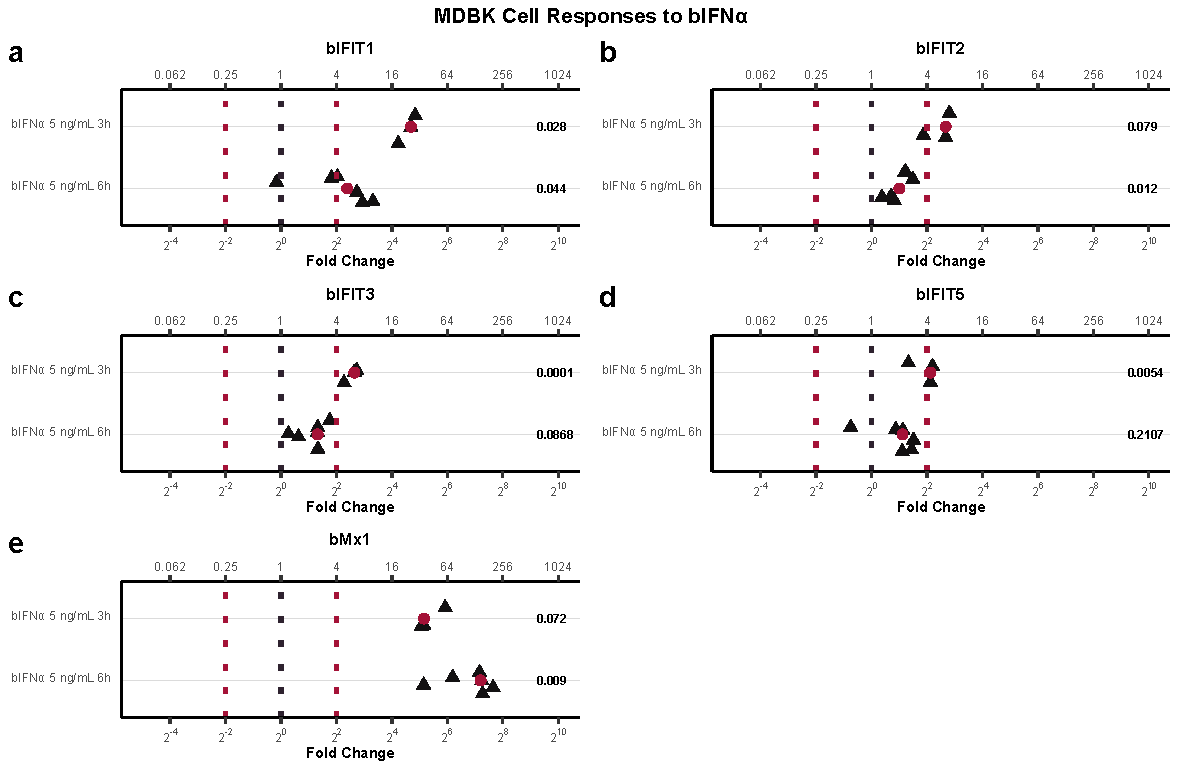
\includegraphics[width=1\linewidth]{07. Chapter 2/Figs/02. Induction/01. mdbk_treat_bifna.pdf}
    \caption[\textit{bIFIT} Gene Expression in MDBK Cells in Response to bIFN\(\alpha\) Stimulation.]{\textbf{\textit{bIFIT} Gene Expression in MDBK Cells in Response to bIFN\(\alpha\) Stimulation.} (a) \textit{bIFIT1}, (b) \textit{bIFIT2}, (c) \textit{bIFIT3}, (d) \textit{bIFIT5}, and (e) \textit{bMx1} gene expression levels were assessed using quantitative real-time PCR (qPCR) in MDBK cells following stimulation with bovine interferon alpha (IFN\(\alpha\)) at a concentration of 5 ng/mL for a treatment duration of either 3 or 6 hours. Relative expression values are normalized to standardized mock-treated samples. Median values are represented by red circles. The black dotted line represents mock expression levels, while the red dotted lines indicate biologically significant induction thresholds. Numeric values indicate the p-values compared to mock-treated samples.}
    \label{fig:MDBK responses to bIFNa}
\end{figure}

Furthermore, we aimed to investigate the involvement of Toll-like Receptor 4 (TLR4) in \textit{bIFIT} induction, previously observed to play a role in the A549 cell line (refer to Figure \ref{fig:A549 Response to LPS} in Section \ref{subsec:Human IFIT Responses to Activators of Innate Immune Response}). MDBK cells were incubated with LPS for 6 hours at concentrations of 0.5, 1, 2.5, 5, and 10 ng/mL. Subsequently, the cells were lysed, and their RNA was extracted, converted to cDNA, and quantified by qPCR as previously described. Our findings indicate that neither \textit{bMx1} nor \textit{bIFITs} were induced to biologically significant levels by LPS within the tested concentration range. Most time points revealed no relative change, while 2.5 ng/mL resulted in a 50\% reduction in the levels of \textit{bIFIT1}, \textit{bIFIT2}, and \textit{bIFIT3}. Evidently, the data suggests that LPS, at the tested concentrations, does not induce \textit{bMx1} or \textit{bIFITs}; if anything, it causes a slight downregulation of their expression. As a side note, while the datasets for \textit{bIFIT3}, \textit{bIFIT5}, and \textit{bMx1} exhibited a normal distribution of data with equal variances, the datasets for \textit{bIFIT1} and \textit{bIFIT2} showed normal distributions with unequal variances.


\begin{figure}
    \centering
    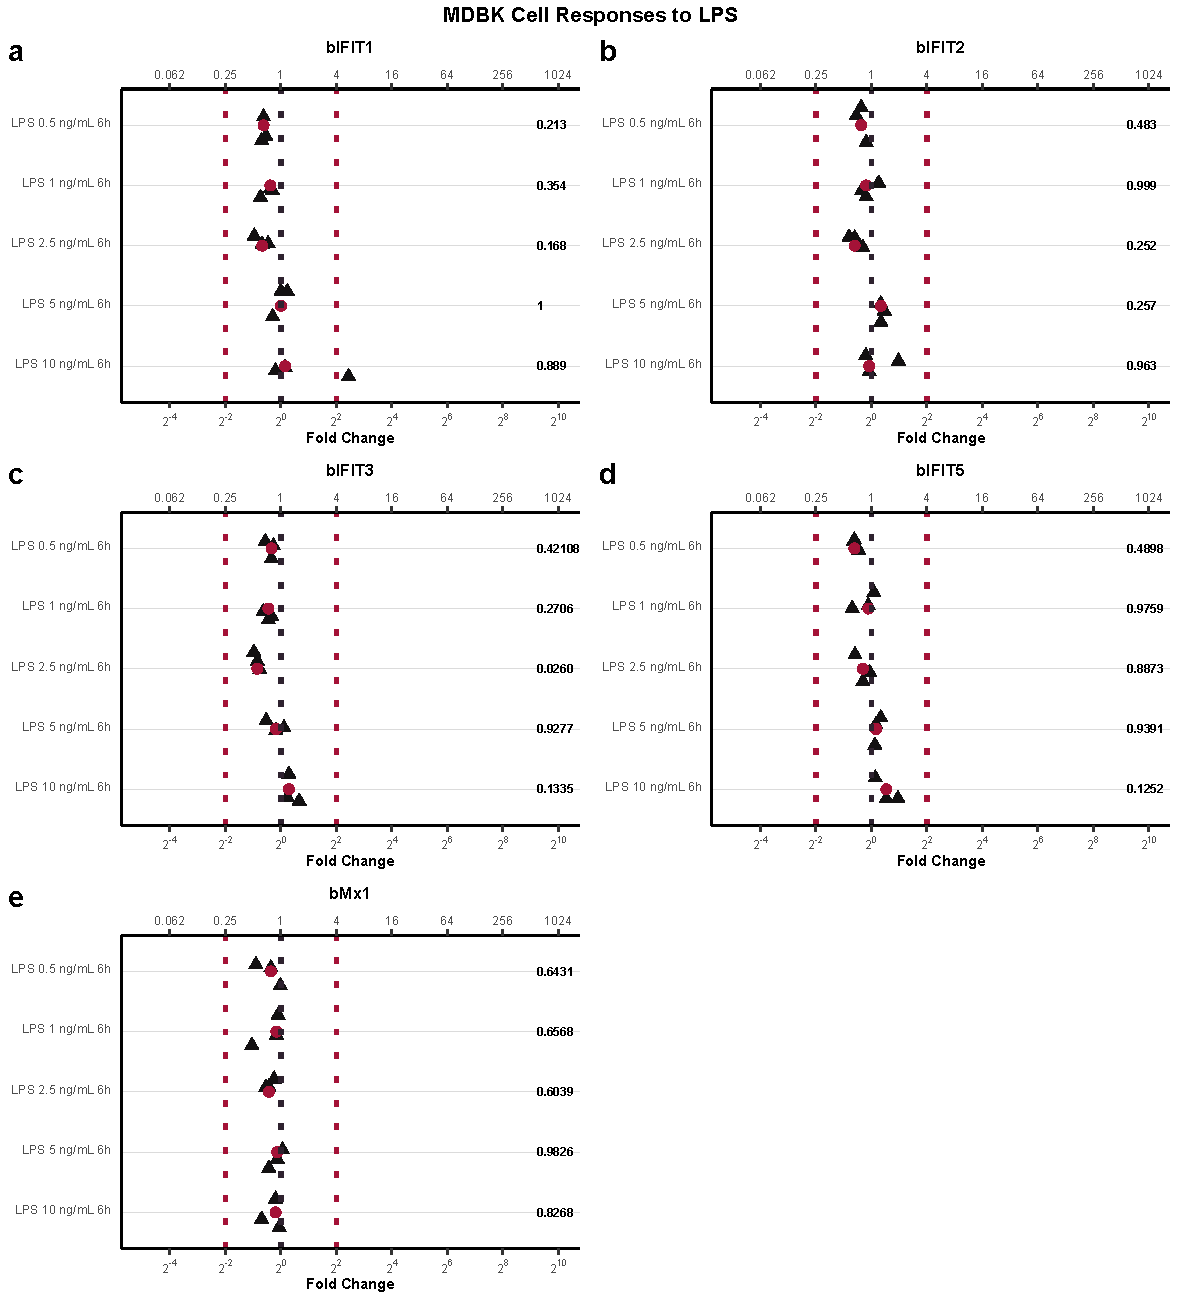
\includegraphics[width=1\linewidth]{07. Chapter 2/Figs/02. Induction/02. mdbk_treat_lps.pdf}
    \caption[\textit{bIFIT} Gene Expression in MDBK Cells in Response to LPS Stimulation.]{\textbf{\textit{bIFIT} Gene Expression in MDBK Cells in Response to LPS Stimulation.} (a) \textit{bIFIT1}, (b) \textit{bIFIT2}, (c) \textit{bIFIT3}, (d) \textit{bIFIT5}, and (e) \textit{bMx1} gene expression levels were assessed using quantitative real-time PCR (qPCR) in MDBK cells following stimulation with bacterial LPS at a concentration of 0.5, 1, 2.5, 5, and 10 ng/mL for a treatment duration of 6 hours. Relative expression values are normalized to standardized mock-treated samples. Median values are represented by red circles. The black dotted line represents mock expression levels, while the red dotted lines indicate biologically significant induction thresholds. Numeric values indicate the p-values compared to mock-treated samples.}
    \label{fig:MDBK responses to LPS}
\end{figure}

To validate the MDBK induction data, the BT cell line was employed. Originating from Bovine viral diarrhea virus (BVDV) negative bovine nasal turbinate cells, isolated in 1974 from a neonatal Holstein cow (\cite{McClurkin1974ComparisonVirus}), these cells, mentioned in Section \ref{Growth Curves of Bovine RSV in Bovine Cell Lines}, facilitate bRSV replication and originate from a more physiologically significant site in the bRSV life cycle compared to the MDBK cell line. BT cells were incubated with 5 ng/mL of bIFN\(\alpha\) for either 3 hours or 24 hours. Figure \ref{fig:BT responses to bifna} depicts the results. At 3 hours of treatment, all genes, except \textit{bIFIT2}, were induced to biologically significant levels. However, after 24 hours, the relative mRNA levels returned to basal levels. Specifically, \textit{bIFIT1} displayed the highest response with a 20-fold induction, followed by \textit{bMx1} with a 16-fold increase. \textit{bIFIT3} showed an 8-fold induction, while \textit{bIFIT5} exhibited a 4-fold increase. Notably, while the dataset for \textit{bIFIT2} displayed a normal distribution of data with equal variances, all other datasets showed normal distributions with unequal variances. In summary, it can be concluded that the BT cell line is sensitive to interferon and competent in \textit{bIFIT} induction. This data aligns with the MDBK data (Figure \ref{fig:MDBK responses to bIFNa}), revealing acute responses of \textit{bIFITs} to bIFN\(\alpha\) stimulation, although the induction is not sustained by 24 hours. Differences include the loss of induction persistence of \textit{bMx1} and the absence of bIFN\(\alpha\) sensitivity in \textit{bIFIT2}.

\begin{figure}
    \centering
    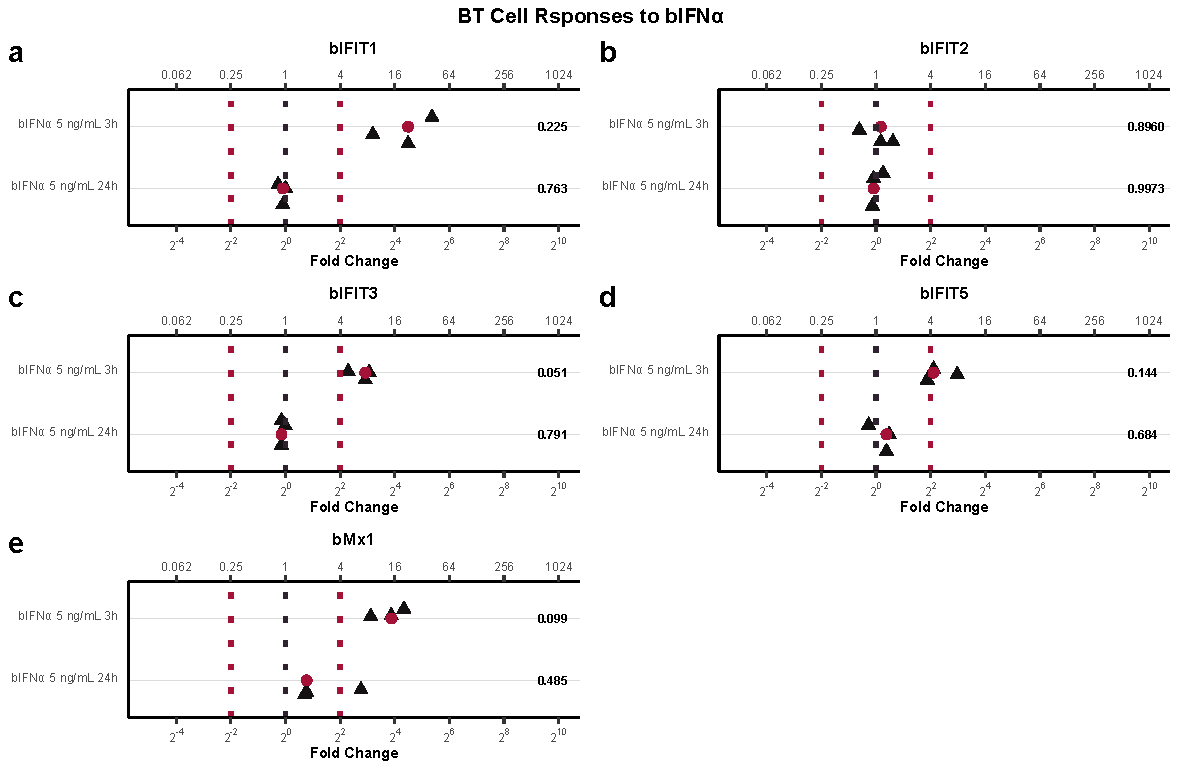
\includegraphics[width=1\linewidth]{07. Chapter 2/Figs/02. Induction/08. bt_bifna.pdf}
    \caption[\textit{bIFIT} Gene Expression in BT Cells in Response to bIFN\(\alpha\) Stimulation.]{\textbf{\textit{bIFIT} Gene Expression in BT Cells in Response to bIFN\(\alpha\) Stimulation.} (a) \textit{bIFIT1}, (b) \textit{bIFIT2}, (c) \textit{bIFIT3}, (d) \textit{bIFIT5}, and (e) \textit{bMx1} gene expression levels were assessed using quantitative real-time PCR (qPCR) in BT cells following stimulation with bovine interferon alpha (IFN\(\alpha\)) at a concentration of 5 ng/mL for a treatment duration of either 3 or 24 hours. Relative expression values are normalized to standardized mock-treated samples. Median values are represented by red circles. The black dotted line represents mock expression levels, while the red dotted lines indicate biologically significant induction thresholds. Numeric values indicate the p-values compared to mock-treated samples.}
    \label{fig:BT responses to bifna}
\end{figure}

\subsection{Bovine \textit{IFITs} Responses to Bovine RSV Infection} \label{subsec:Bovine IFITs Responses to Bovine RSV Infection}
Confirming the competence of the selected cell lines for \textit{bIFIT} induction, our goal was to evaluate the impact of bRSV infection on \textit{bIFIT} induction, particularly concerning varying viral MOIs and infection durations. To achieve this, MDBK cells were infected with crudely extracted bRSV at MOIs of 0.1, 1, and 2 for durations of 24 and 48 hours post-infection (HPI). The viruses employed in these experiments were prepared and quantified as detailed in Section \ref{subsec:Virus Propagation and Production} and Section \ref{subsec:Virus Quantification by TCID50 Assay}.

\begin{figure}
    \centering
    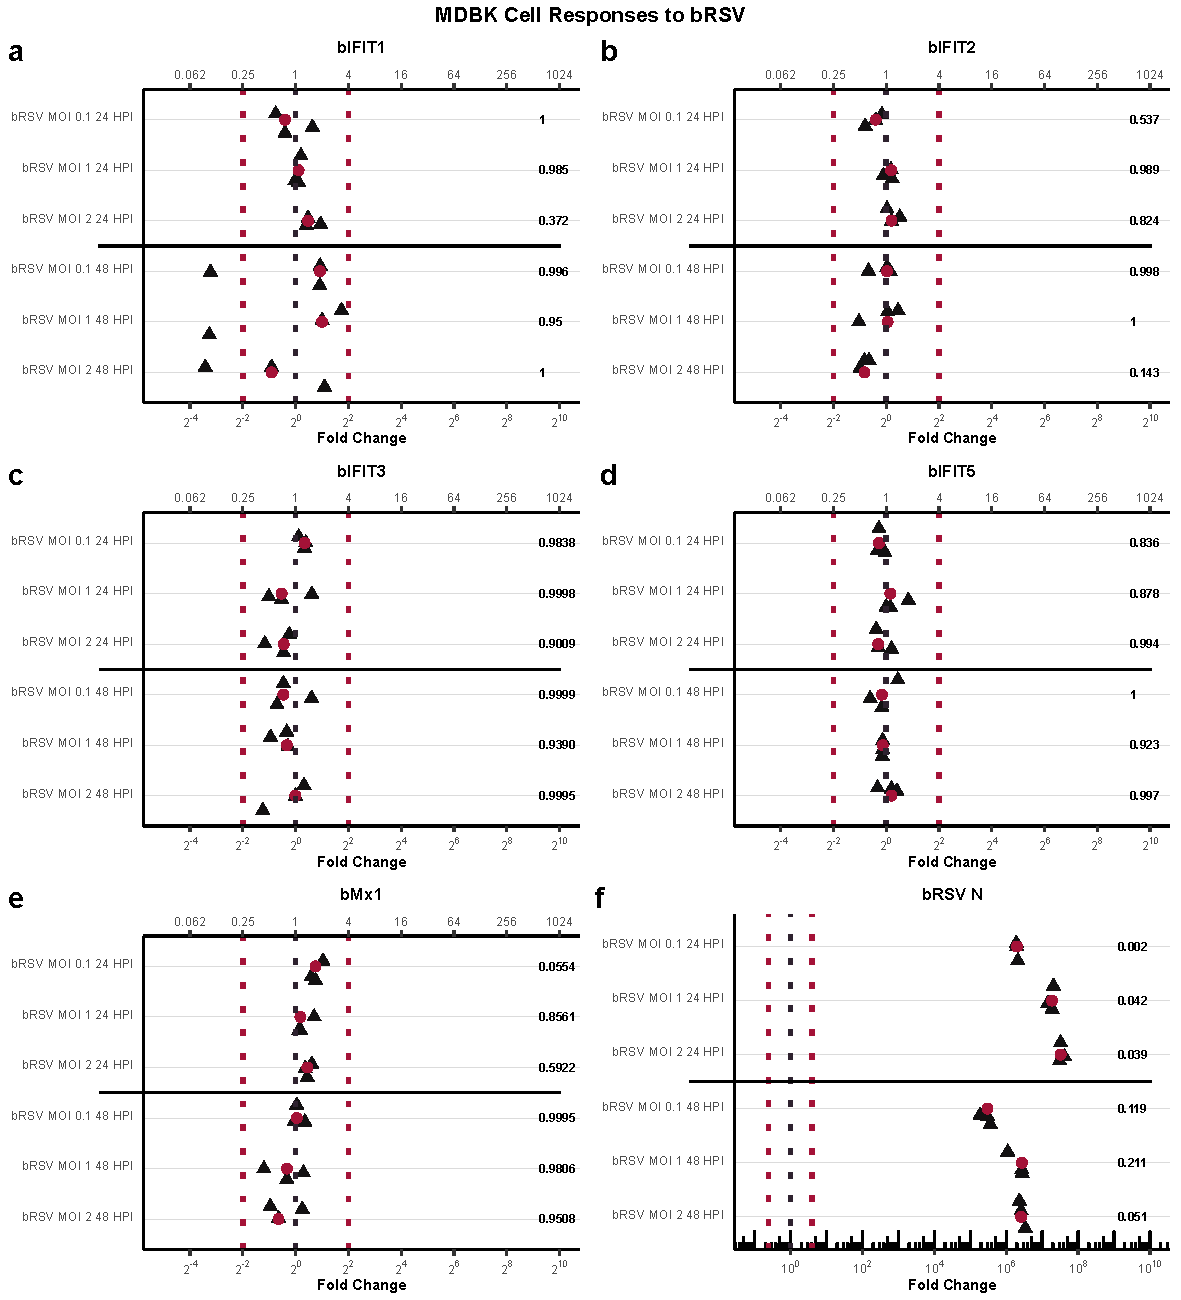
\includegraphics[width=1\linewidth]{07. Chapter 2/Figs/02. Induction/03. mdbk_brsv_timepoints.pdf}
    \caption[MDBK \textit{bIFIT} Response to bRSV Infection as a Function of Time and MOI.]{\textbf{MDBK \textit{bIFIT} Response to bRSV Infection as a Function of Time and MOI.} (a) \textit{bIFIT1}, (b) \textit{bIFIT2}, (c) \textit{bIFIT3}, (d) \textit{bIFIT5}, (e) \textit{bMx1} and (f) \textit{bRSV N} gene expression levels were assessed using quantitative real-time PCR (qPCR) in MDBK cell line following infection with bovine RSV at MOI of either 0.1, 1, or 2 for either 24 or 48 hours post-infection. Relative expression values are normalized to standardized mock-treated samples. Median values are represented by red circles. The black dotted line represents mock expression levels, while the red dotted lines indicate biologically significant induction thresholds. Numeric values indicate the p-values compared to mock-treated samples.}
    \label{fig:MDBK responses to bRSV timepoints}
\end{figure}

The results of this experiment are depicted in Figure \ref{fig:MDBK responses to bRSV timepoints}. Evidently, while bRSV demonstrated successful replication, as indicated by the notably high relative \textit{bRSV N} values across all tested MOIs and timepoints (panel f), there were no biologically significant alterations in the mRNA levels of either \textit{bMx1} or \textit{bIFITs}. Specifically, while the mRNA levels of \textit{bIFIT3} and \textit{bIFIT5} remained unchanged under all conditions, minor positive and negative changes were observed in the expression of the other genes. Notably, \textit{bIFIT1} levels doubled for infections at 0.1 and 1 MOI at 48 HPI but decreased by half at MOI 2 at 48 HPI. \textit{bIFIT2} mRNA levels showed no significant changes except for the 2 MOI infection at 48 HPI. Additionally, \textit{bMx1} exhibited a two-fold induction in the case of 0.1 MOI infection at 24 HPI and a 50\% downregulation after 2 MOI infection at 48 HPI. From a statistical standpoint, the datasets for \textit{bIFIT3} and \textit{bMx1} showcased normal distributions and equal variances, while the others exhibited normal distributions with unequal variances. The minimal responses to bRSV infection are intriguing, particularly considering our human data from Chapter \ref{ch:Assessment of Transcriptional Induction of Human IFITs in the Context of RSV}, which indicates that the \textit{hIFIT} responses are predominantly mediated by IFN\(\alpha\). Furthermore, as discussed in Section \ref{subsec:Bovine IFIT Responses to Activators of Innate Immune Response}, we are aware that \textit{bIFITs}, especially \textit{bMx1}, respond to bovine IFN\(\alpha\) stimulation. It is plausible that certain constituents within the bRSV or specific cytokines or chemokines in the crudely extracted bRSV preparations might impede the cascades necessary for \textit{bIFIT} induction.

\begin{figure}
    \centering
    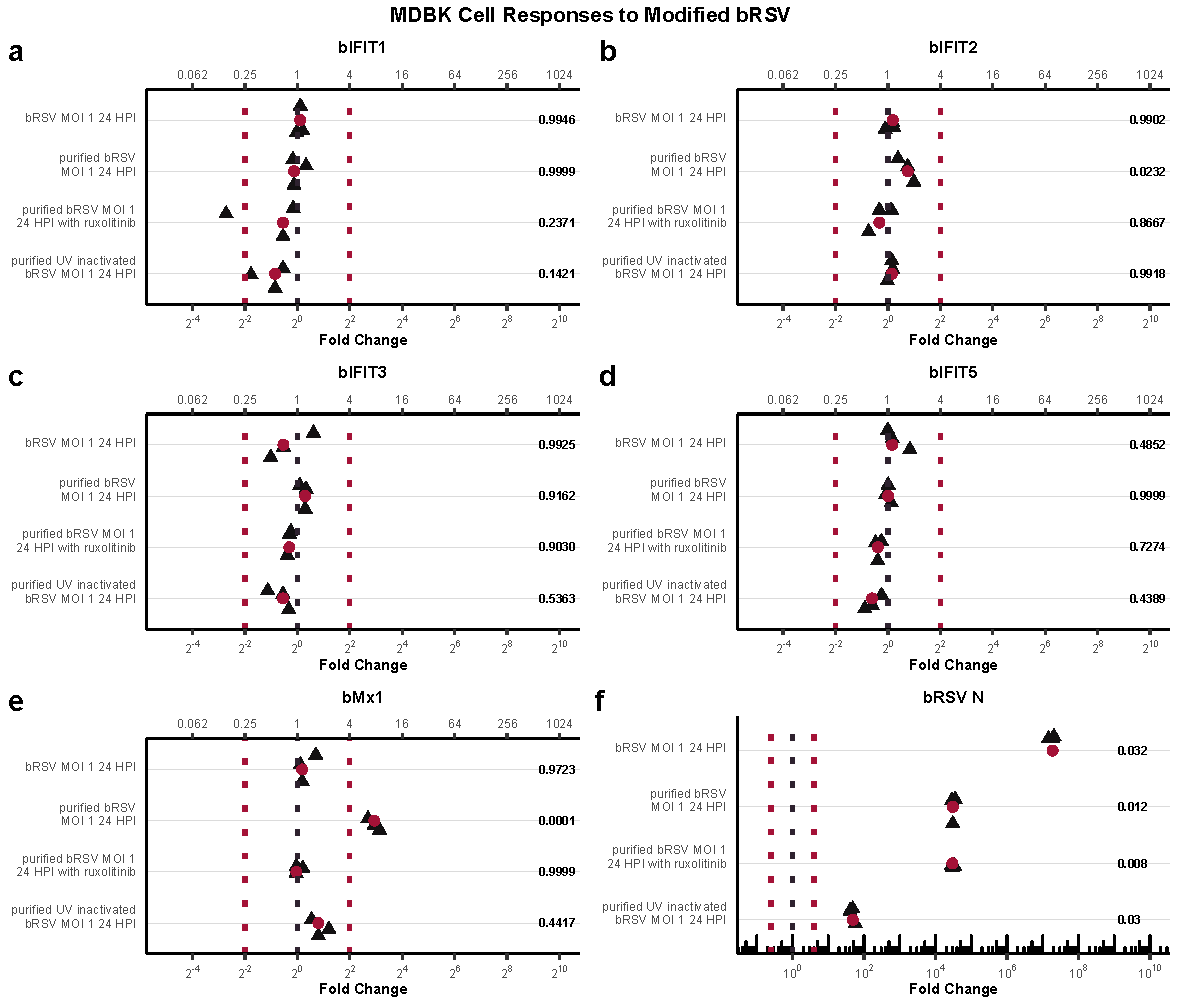
\includegraphics[width=1\linewidth]{07. Chapter 2/Figs/02. Induction/04. mdbk_brsv_uv_roxo.pdf}
    \caption[Impact of Ultra-Purification, UV-Inactivation, and INFR Inhibition on \textit{bIFIT} Induction in MDBK Cells Following bRSV Infection.]{\textbf{Impact of Ultra-Purification, UV-Inactivation, and INFR Inhibition on \textit{bIFIT} Induction in MDBK Cells Following bRSV Infection.} (a) \textit{bIFIT1}, (b) \textit{bIFIT2}, (c) \textit{bIFIT3}, (d) \textit{bIFIT5}, (e) \textit{bMx1}, and (f) \textit{bRSV N} gene expression levels were assessed using quantitative real-time PCR (qPCR) in MDBK cell line following infection with ultra-purified bRSV at MOI 1 for 24 hours. The cells were subjected to three different conditions: virus infection alone (top row), virus infection in the presence of 5 nM of ruxolitinib (interferon receptor inhibitor) throughout the infection (middle row), or UV-inactivated bRSV infection (bottom row). Relative expression values are normalized to standardized mock-treated samples. Median values are represented by red circles. The black dotted line represents mock expression levels, while the red dotted lines indicate biologically significant induction thresholds. Numeric values indicate the p-values compared to mock-treated samples.}
    \label{fig:The effect of ultra-purification, UV-inactivation and INFR inhibition on hIFIT induction following hRSV infection in MDBK}
\end{figure}

To investigate the possible influence of cellular contaminants on gene induction, MDBK cells were infected with ultrapurified bRSV, prepared through ultra-centrifugation on a discontinuous sucrose cushion as outlined in Section \ref{subsec:Virus Propagation and Production}. Simultaneously, we aimed to evaluate the impact of pharmacological inhibition of the interferon receptor and physical inactivation of bRSV on \textit{bIFIT} and \textit{bMx1} induction. This approach was prompted by our prior observation, as described in Section \ref{subsec:Human IFITs Responses to Human RSV} and illustrated in Figure \ref{fig:The effect of ultra-purification, UV-inactivation and INFR inhibition on hIFIT induction following hRSV infection in BEAS2B}, suggesting the requirement of basal interferon receptor activation for the maintenance of basal \textit{hIFIT} mRNA expression. The resultant data is displayed in Figure \ref{fig:The effect of ultra-purification, UV-inactivation and INFR inhibition on hIFIT induction following hRSV infection in MDBK}. Interestingly, the purification status of the virus did not influence the induction of \textit{bIFITs}. However, ultrapurification led to a seven-fold induction of \textit{bMx1}, a response that was entirely reversed by the presence of the interferon receptor inhibitor, ruxolitinib. Moreover, the presence of ruxolitinib marginally reduced the abundance of all \textit{bIFIT} mRNAs, though not to biologically significant levels. Intriguingly, the relative median \textit{bRSV N} mRNA value remained consistent between the first two conditions, contrary to our observations in human samples where the presence of ruxolitinib amplified the relative median \textit{bRSV N} mRNA. Additionally, UV-inactivation of bRSV resulted in only minor changes for all genes, approximately around \(\pm\)2 in magnitude. Overall, the induction response of \textit{bMx1} mirrors what was observed with human RSV in A549 and BEAS2B cell lines in Chapter \ref{ch:Assessment of Transcriptional Induction of Human IFITs in the Context of RSV}. Conversely, we did not observe any significant alterations in the mRNA levels of \textit{bIFITs}. This suggests that certain cellular contaminants present in crudely extracted bRSV preparations were suppressing the induction of \textit{bMx1}, whereas their absence had no bearing on the potential inhibition of \textit{bIFIT} induction. In terms of data distribution, while \textit{bRSV N} and \textit{bMx1} datasets exhibited normal distributions with unequal variances, the datasets for \textit{bIFIT1}, \textit{bIFIT2}, \textit{bIFIT3}, and \textit{bIFIT5} displayed normal distributions with equal variances.

\begin{figure}
    \centering
    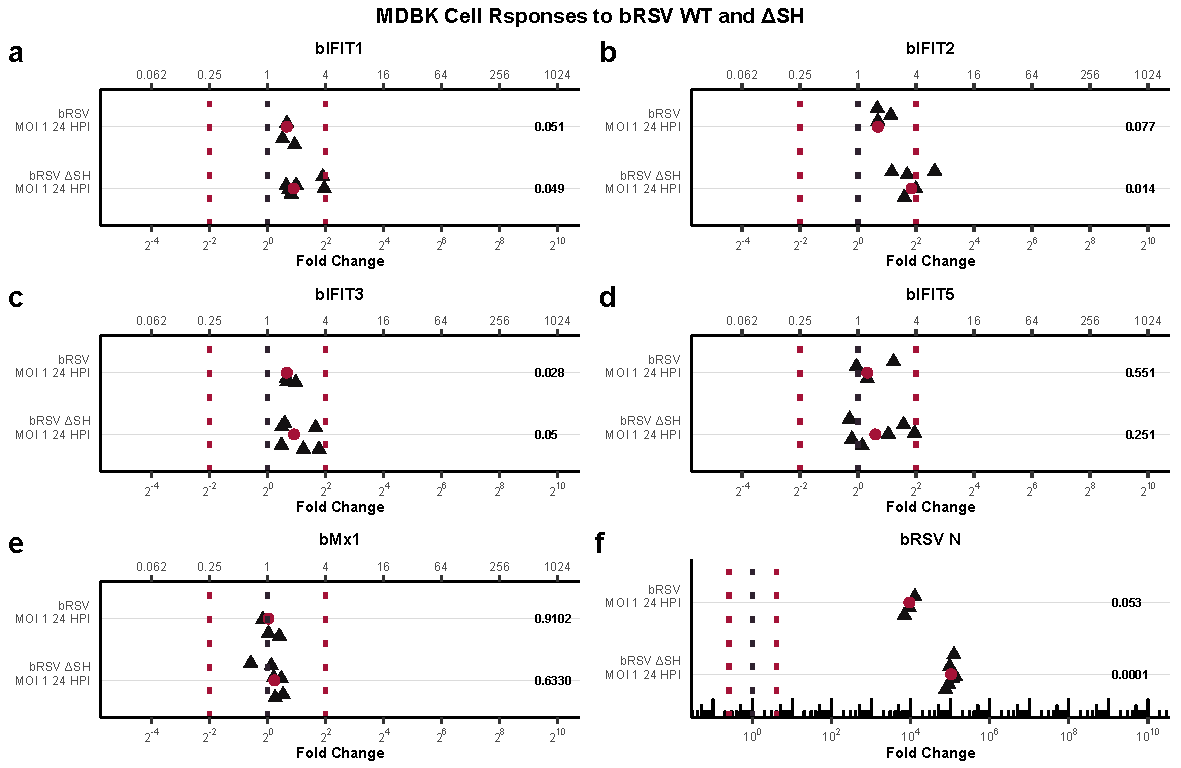
\includegraphics[width=1\linewidth]{07. Chapter 2/Figs/02. Induction/05. mdbk_brsv_moi1_dsh.pdf}
    \caption[MDBK \textit{bIFIT} Response to WT and \(\Delta\)SH bRSV Infection.]{\textbf{MDBK \textit{bIFIT} Response to WT and \(\Delta\)SH bRSV Infection.} (a) \textit{bIFIT1}, (b) \textit{bIFIT2}, (c) \textit{bIFIT3}, (d) \textit{bIFIT5}, (e) \textit{bMx1}, and (f) \textit{bRSV N} gene expression levels were assessed using quantitative real-time PCR (qPCR) in MDBK cell line following infection with WT or \(\Delta\)SH bRSV at MOI 1 for 24 hours post-infection. Relative expression values are normalized to standardized mock-treated samples. Median values are represented by red circles. The black dotted line represents mock expression levels, while the red dotted lines indicate biologically significant induction thresholds. Numeric values indicate the p-values compared to mock-treated samples.}
    \label{fig:MDBK responses to dSH}
\end{figure}

Next, we sought to determine whether any of the bRSV genes inhibit the induction of \textit{bIFITs} or remain uninvolved during bRSV infection. As presented in Section \ref{subsec:Genomic and Virion Composition}, RSV proteins SH, NS1, and NS2 are known for their inhibitory actions on innate immune pathways through their interactions with constituents (cite the relevant source and update the information). Our hypothesis posits that these proteins impede the induction of \textit{bIFITs}. Utilizing a panel of bRSV deletion mutants, including bRSV \(\Delta\)SH, \(\Delta\)NS1, \(\Delta\)NS2, and the double deletion mutant \(\Delta\)NS1/2, we sought to investigate this hypothesis. These viruses were propagated and quantified as detailed in Section \ref{subsec:Virus Propagation and Production} and Section \ref{subsec:Virus Quantification by TCID50 Assay}. The absence of non-structural proteins led to decreased final titers, hence we could only infect at much lower MOIs.

Subsequently, MDBK cells were infected with MOI 1 WT and \(\Delta\)SH bRSV for 24 hours. Figure \ref{fig:MDBK responses to dSH} portrays the relative mRNA changes of \textit{bIFITs} and \textit{bMx1} extracted from MDBK cells 24 HPI with MOI 1 WT and \(\Delta\)SH bRSV. Both viruses demonstrated successful replication, with \(\Delta\)SH bRSV exhibiting higher median relative mRNA levels at the experiment's endpoint compared to WT bRSV, contradicting the expected decreased fitness of this virus. However, \textit{bIFITs} and \textit{bMx1} responses to crudely extracted WT bRSV remained consistent with previous minimal responses to the infection (see Figure \ref{fig:MDBK responses to bRSV timepoints}). Notably, \(\Delta\)SH bRSV infection elicited no differential responses for any tested genes compared to WT bRSV infection, except for \textit{bIFIT2}, where median relative mRNA abundance increased to biologically significant levels at 4-fold. Regarding data distribution, the \textit{bMx1} dataset exhibited a normal distribution of data with equal variances, while \textit{bIFIT1}, \textit{bIFIT2}, \textit{bIFIT3}, \textit{bIFIT5}, and \textit{bRSV N} datasets exhibited normal distributions with unequal variances.

\begin{figure}
    \centering
    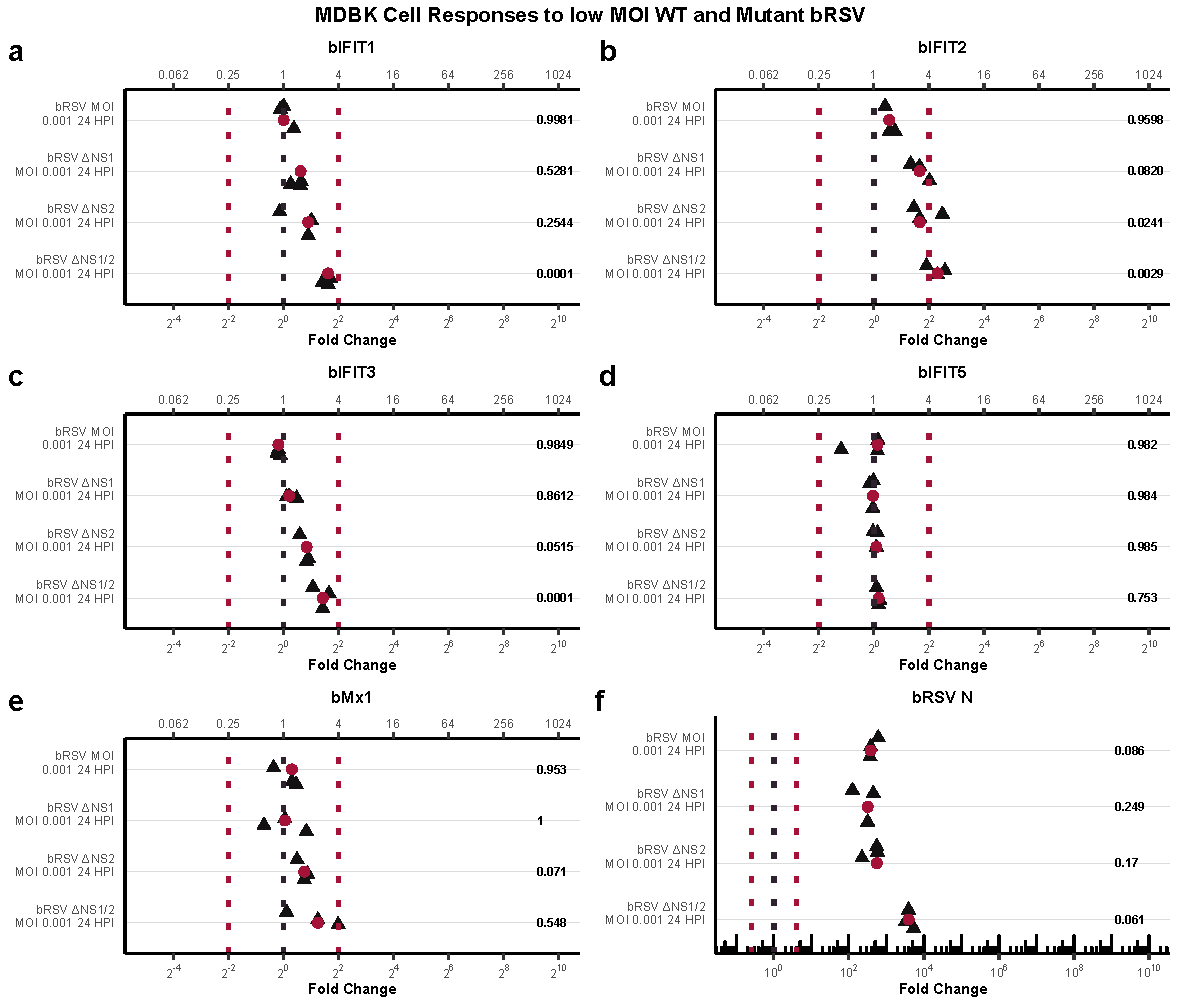
\includegraphics[width=1\linewidth]{07. Chapter 2/Figs/02. Induction/06. mdbk_brsv_low_moi.pdf}
    \caption[MDBK \textit{bIFIT} Response to Low MOI bRSV Infections.]{\textbf{MDBK \textit{bIFIT} Response to Low MOI bRSV Infections.} (a) \textit{bIFIT1}, (b) \textit{bIFIT2}, (c) \textit{bIFIT3}, (d) \textit{bIFIT5}, (e) \textit{bMx1}, and (f) \textit{bRSV N} gene expression levels were assessed using quantitative real-time PCR (qPCR) in MDBK cell line following infection with WT or \(\Delta\)NS1, \(\Delta\)NS2, and \(\Delta\)NS1/2 bRSV at MOIs of 0.001 for 24 hours post-infection. Relative expression values are normalized to standardized mock-treated samples. Median values are represented by red circles. The black dotted line represents mock expression levels, while the red dotted lines indicate biologically significant induction thresholds. Numeric values indicate the p-values compared to mock-treated samples.}
    \label{fig:MDBK responses to low MOI mutant bRSV}
\end{figure}

Continuing the investigation, we utilized 0.001 MOI \(\Delta\)NS1, \(\Delta\)NS2, and \(\Delta\)NS1/2 bRSV along with 0.001 MOI WT bRSV as a control to assess their potential involvement in the suppression of \textit{bIFIT} induction. As illustrated in Figure \ref{fig:MDBK responses to low MOI mutant bRSV}, none of the genes of interest were influenced by WT infection, in line with our previous observations. Concerning the mutant viruses, \textit{bIFIT5} was unresponsive to any of them, while the other genes exhibited marginal induction in at least one condition. Notably, \(\Delta\)NS1 infection influenced only \textit{bIFIT2}, inducing it nearly to biologically significant levels at around 3.8-fold. The absence of NS2 protein caused minor induction in all tested genes, except for \textit{bIFIT5}, approximately a 2-fold increase for \textit{bIFIT1}, \textit{bIFIT3}, and \textit{bMx1}, and a 3.8-fold induction for \textit{bIFIT2}. The infection with the double deletion mutant \(\Delta\)NS1/2 bRSV resulted in the most robust response, inducing \textit{bIFIT1} and \textit{bIFIT3} at 3.8-fold, \textit{bMx1} at 3-fold, and notably, a biologically significant induction of \textit{bIFIT2} at 5-fold. Regarding data distribution, the \textit{bIFIT5}, \textit{bRSV N}, and \textit{bMx1} datasets exhibited a normal distribution of data with unequal variances, while the \textit{bIFIT1}, \textit{bIFIT2}, and \textit{bIFIT3} datasets exhibited normal distributions with equal variances. This data suggests that, except for \textit{bIFIT5}, bRSV NS proteins negatively influence the induction of \textit{bIFITs} and \textit{bMx1}, with NS2 seemingly a more potent inhibitor.

\begin{figure}
    \centering
    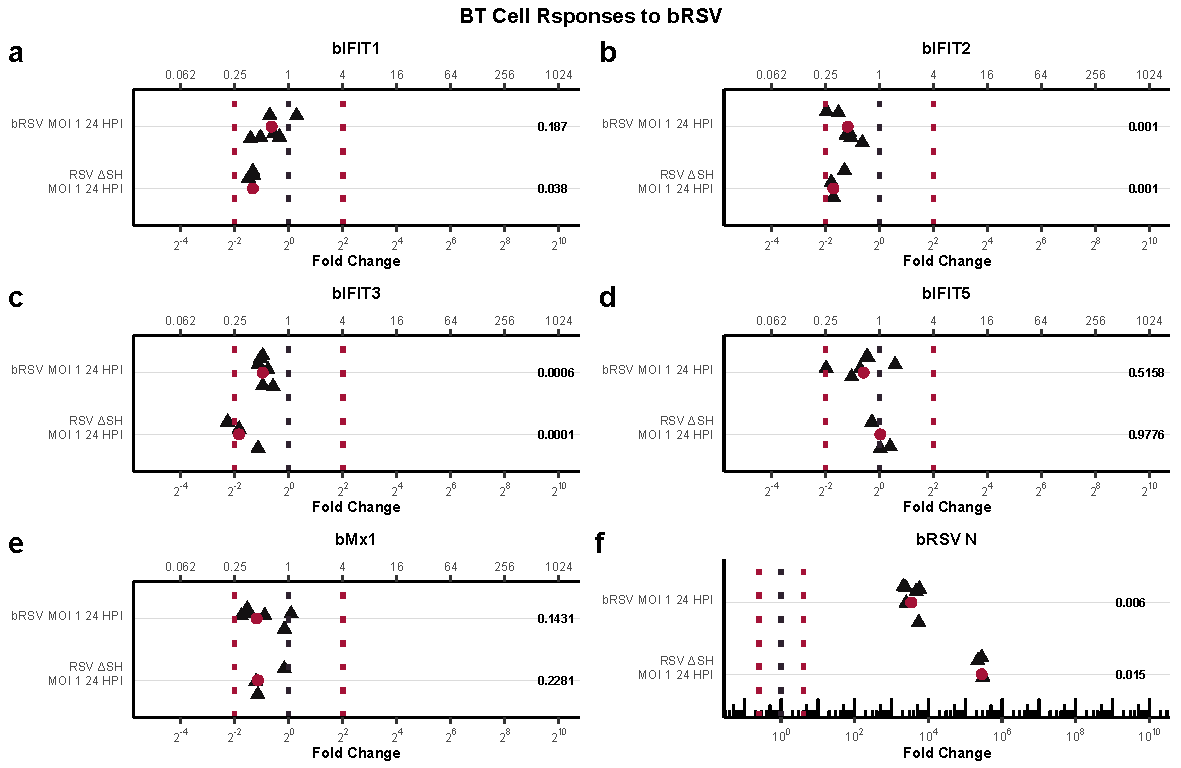
\includegraphics[width=1\linewidth]{07. Chapter 2/Figs/02. Induction/09. bt_brsv.pdf}
    \caption[BT \textit{bIFIT} Response to WT and \(\Delta\)SH bRSV Infection.]{\textbf{BT \textit{bIFIT} Response to WT and \(\Delta\)SH bRSV Infection.} (a) \textit{bIFIT1}, (b) \textit{bIFIT2}, (c) \textit{bIFIT3}, (d) \textit{bIFIT5}, (e) \textit{bMx1}, and (f) \textit{bRSV N} gene expression levels were assessed using quantitative real-time PCR (qPCR) in BT cell line following infection with WT or \(\Delta\)SH bRSV at MOI 1 for 24 hours post-infection. Relative expression values are normalized to standardized mock-treated samples. Median values are represented by red circles. The black dotted line represents mock expression levels, while the red dotted lines indicate biologically significant induction thresholds. Numeric values indicate the p-values compared to mock-treated samples.}
    \label{fig:BT responses to bRSV}
\end{figure}

Finally, we aimed to partially validate the bRSV infection data using the BT cell line. The cells were infected with crudely extracted WT and \(\Delta\)SH bRSV at an MOI of 1 for 24 hours. The relevant data is depicted in Figure \ref{fig:BT responses to bRSV}. It's noteworthy that all datasets exhibited normal distribution and equal variance except for \textit{bIFIT1} and \textit{bRSV N}. In general, a reduction in mRNA levels was observed as a consequence of infection, regardless of the virus used. Specifically, WT bRSV infection led to a \(2^{-0.5}\)-fold decrease for \textit{bIFIT1} and \textit{bIFIT5}, a \(2^{-1}\)-fold decrease for \textit{bIFIT2} and \textit{bIFIT3}, and a \(2^{-1.5}\)-fold decrease for \textit{bMx1}. Infection with \(\Delta\)SH bRSV resulted in approximately a \(2^{-1.5}\)-fold decrease in the levels of \textit{bIFIT1} and \textit{bMx1}, a biologically significant decrease of \(2^{-2}\)-fold for \textit{bIFIT2} and \textit{bIFIT3}, and no alteration in \textit{bIFIT5} mRNA levels. Overall, the presence of the SH protein appears to stimulate the induction of \textit{bIFIT} and \textit{bMx1}. This contrasts with observations in the MDBK cell line, where no differences were observed in the induction potential of WT and \(\Delta\)SH bRSV, except for \textit{bIFIT2}, which was significantly upregulated in the absence of the SH protein (Figure \ref{fig:MDBK responses to dSH}).

\subsection{Bovine \textit{IFITs} Responses to hRSV Infection} \label{subsec:Bovine IFITs Responses to hRSV Infection}
We sought to investigate potential cross-species protection between hRSV and bRSV. As detailed in Section \ref{subsec:Human IFITs Responses to bRSV}, bRSV induces \textit{hIFITs} to a level surpassing that of equivalent hRSV infection in the A549 cell line, suggesting cross-protection of human cells to both viruses. While minimal \textit{bIFIT} or \textit{bMx1} responses were observed to WT or mutant bRSV infections in the MDBK and BT cell lines, we aimed to assess the potential response to hRSV. Furthermore, as noted in Section \ref{subsec:Human IFITs Responses to Human RSV}, the purification methodology for isolating hRSV influenced \textit{hIFIT} induction, with ultrapurified preparations causing higher levels of induction. Considering these factors, MDBK and BT cells were infected with crude extracted and ultracentrifugation-purified hRSV at an MOI of 1 for 24 hours. Subsequently, cells were lysed, mRNA was extracted and converted into cDNA, and transcripts were quantified using RT-qPCR.

\begin{figure}
    \centering
    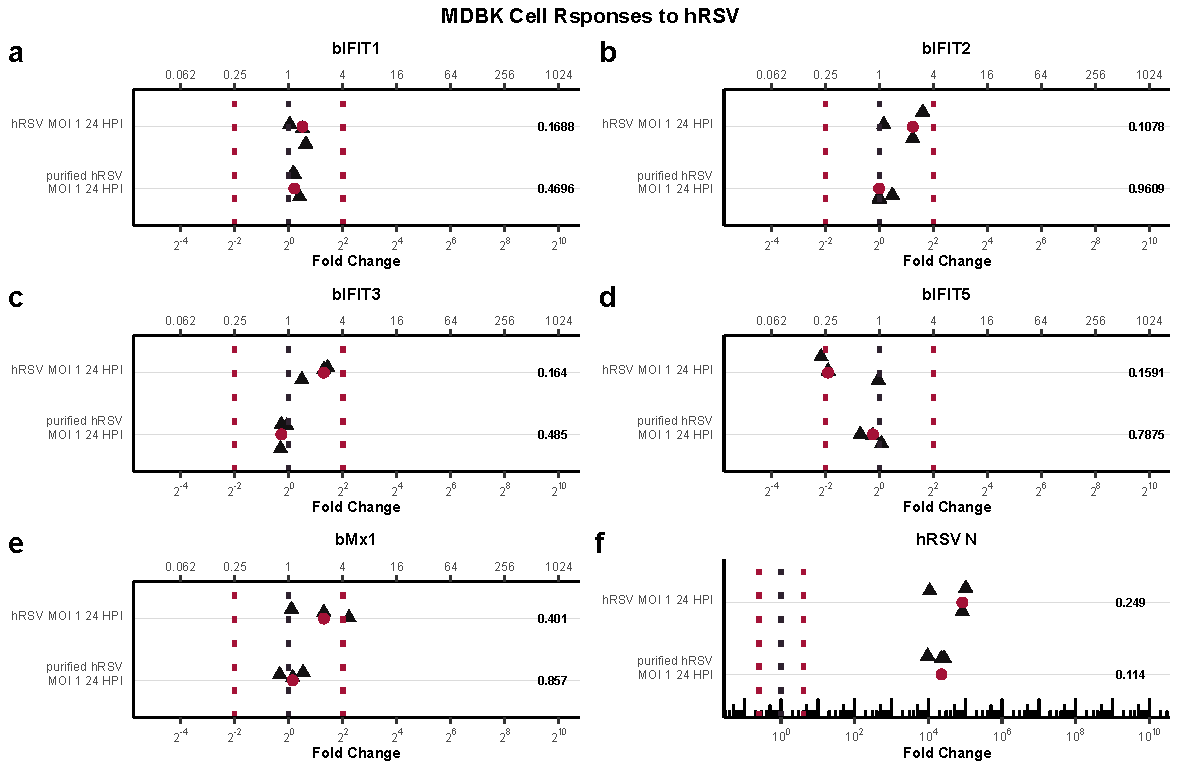
\includegraphics[width=1\linewidth]{07. Chapter 2/Figs/02. Induction/07. mdbk_hrsv.pdf}
    \caption[MDBK \textit{bIFIT} Response to Crude-Extracted and Ultra-Purified hRSV Infection.]{\textbf{MDBK \textit{bIFIT} Response to Crude-Extracted and Ultra-Purified hRSV Infection.} (a) \textit{bIFIT1}, (b) \textit{bIFIT2}, (c) \textit{bIFIT3}, (d) \textit{bIFIT5}, (e) \textit{bMx1}, and (f) \textit{hRSV N} gene expression levels were assessed using quantitative real-time PCR (qPCR) in MDBK cell line following infection with crude-extraccted and ultra-purified hRSV at MOI 1 for 24 hours post-infection. Relative expression values are normalized to standardized mock-treated samples. Median values are represented by red circles. The black dotted line represents mock expression levels, while the red dotted lines indicate biologically significant induction thresholds. Numeric values indicate the p-values compared to mock-treated samples.}
    \label{fig:bIFIT responses to hRSV infection in MDBK}
\end{figure}

Figure \ref{fig:bIFIT responses to hRSV infection in MDBK} illustrates the responses of \textit{bIFITs} and \textit{bMx1} to hRSV in MDBK cells. Both viral preparations successfully replicated, as evidenced by the quantification of \textit{hRSV N} (Panel f; \(2^{5}\)-fold and \(2^{4.2}\)-fold increases, respectively), albeit unexpectedly exhibiting an order of magnitude difference in the final fold changes. Notably, ultrapurified hRSV infection did not influence the relative levels of any tested genes. In contrast, crude extracted hRSV infection induced a variety of effects: a modest induction of \textit{bIFIT1} by 1.5-fold, and \textit{bIFIT2}, \textit{bIFIT3}, and \textit{bMx1} by 3-fold, alongside a significant downregulation of \textit{bIFIT5} by \(2^{-2}\)-fold. The datasets for \textit{bIFIT1}, \textit{bIFIT2}, and \textit{bIFIT3} exhibited normal distribution with equal variances, while the rest displayed normal distributions with unequal variances.

\begin{figure}
    \centering
    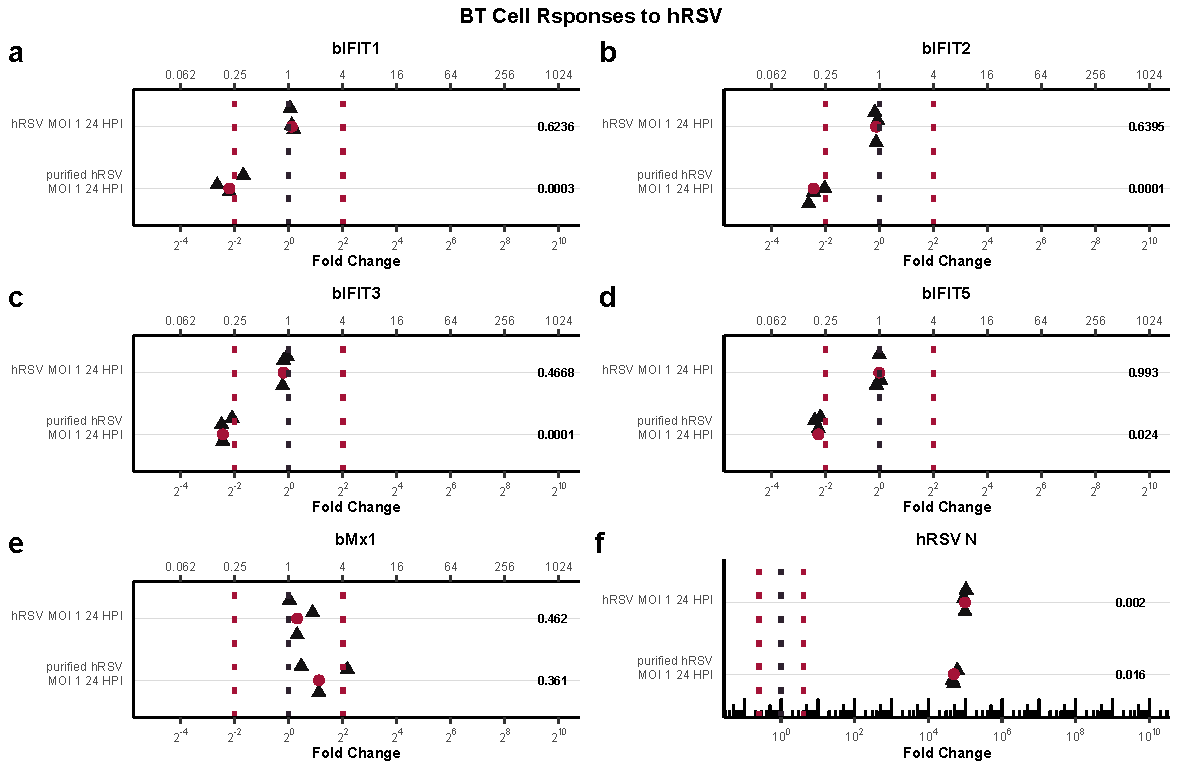
\includegraphics[width=1\linewidth]{07. Chapter 2/Figs/02. Induction/10. bt_hrsv.pdf}
    \caption[BT \textit{bIFIT} Response to Crude-Extracted and Ultra-Purified hRSV Infection.]{\textbf{BT \textit{bIFIT} Response to Crude-Extracted and Ultra-Purified hRSV Infection.} (a) \textit{bIFIT1}, (b) \textit{bIFIT2}, (c) \textit{bIFIT3}, (d) \textit{bIFIT5}, (e) \textit{bMx1}, and (f) \textit{hRSV N} gene expression levels were assessed using quantitative real-time PCR (qPCR) in BT cell line following infection with crude-extraccted and ultra-purified hRSV at MOI 1 for 24 hours post-infection. Relative expression values are normalized to standardized mock-treated samples. Median values are represented by red circles. The black dotted line represents mock expression levels, while the red dotted lines indicate biologically significant induction thresholds. Numeric values indicate the p-values compared to mock-treated samples.}
    \label{fig:Bt responses to hRSV}
\end{figure}

Results from BT cells infected with hRSV are depicted in Figure \ref{fig:Bt responses to hRSV}. Similar to MDBK cells, hRSV successfully infected and replicated in BT cells. Interestingly, the effect observed in MDBK cells (Figure \ref{fig:bIFIT responses to hRSV infection in MDBK}) was reversed: the crude extracted viral preparation did not influence the expression of the genes of interest, while ultra-purified hRSV caused significant effects. It led to a biologically substantial downregulation of \textit{bIFIT1}, \textit{bIFIT2}, \textit{bIFIT3}, and \textit{bIFIT5} by \(2^{-2.5}\)-fold, and induced \textit{bMx1} by 2-fold. Normal distribution with equal variances was observed for \textit{bIFIT1} and \textit{bIFIT2} datasets, while the others exhibited normal distributions with unequal variances.

\section{Discussion} \label{sec:Discussion Chapter2}
Recap bovine

\lipsum[1-6]


\nomenclature[z-IU]{IU}{International Units}